\chapter{图}

\section{图}

\subsection{图(Graph)}

你的微信中有若干好友,而你的好友又有若干好友。许许多多的用户组成了一个多对多的关系网,这个关系网就是数据结构中的图。\\

再例如使用地图导航功能时,导航会根据你的出发地和目的地规划最佳的地铁换乘路线。许许多多的地铁站组成的交通网络也可以认为是图。\\

图是一种比树更为复杂的数据结构。树的结点之间是一对多的关系,并且存在父与子的层级划分。而图的顶点之间是多对多关系,并且所有顶点都是平等的,无所谓谁是父子。\\

在图中,最基本的单元是顶点(vertex),相当于树中的结点。顶点之间的关联关系被称为边(edge)。图中包含一组顶点和一组边,通常用V表示顶点集合,用E表示边集合。边可以看作是顶点对,即$ (v, w) \in E,\ v, w \in V $。\\

在有些图中,每一条边并不是完全等同的。例如地铁线路,站与站之间的距离都有可能不同。因此图中会涉及边的权重(weight),涉及到权重的图被称为带权图(weighted graph),也称为网络。

\begin{figure}[H]
	\centering
	\begin{tikzpicture}
		\begin{scope}[every node/.style={circle,thick,draw}]
			\node (A) at (0,0) {A};
			\node (B) at (0,3) {B};
			\node (C) at (2.5,4) {C};
			\node (D) at (2.5,1) {D};
			\node (E) at (2.5,-3) {E};
			\node (F) at (5,3) {F};
		\end{scope}

		\begin{scope}[>={Stealth[black]},
			every node/.style={fill=white,circle},
			every edge/.style={draw=black,very thick}]
			\path [-] (A) edge node {5} (B);
			\path [-] (B) edge node {3} (C);
			\path [-] (A) edge node {4} (D);
			\path [-] (D) edge node {3} (C);
			\path [-] (A) edge node {3} (E);
			\path [-] (D) edge node {3} (E);
			\path [-] (D) edge node {3} (F);
			\path [-] (C) edge node {5} (F);
			\path [-] (E) edge node {8} (F);
		\end{scope}
	\end{tikzpicture}
	\caption{带权图}
\end{figure}

还有一种图,顶点之间的关联并不是完全对称的。拿微信举例,你的好友列表里有我,但我的好友列表里未必有你。\\

这样一来,顶点之间的边就有了方向的区分,这种带有方向的图被称为有向图(directed graph)。有向边可以使用<v, w>表示从v指向w的边。\\

\begin{figure}[H]
	\centering
	\begin{tikzpicture}
		\begin{scope}[every node/.style={circle,thick,draw}]
			\node (A) at (0,0) {A};
			\node (B) at (0,3) {B};
			\node (C) at (2.5,4) {C};
			\node (D) at (2.5,1) {D};
			\node (E) at (5,0) {E};
		\end{scope}

		\begin{scope}[>={Stealth[black]},
			every node/.style={fill=white,circle},
			every edge/.style={draw=black,very thick}]
			\path [<->] (A) edge node {5} (B);
			\path [->] (B) edge node {3} (C);
			\path [->] (A) edge node {4} (D);
			\path [<->] (D) edge node {3} (C);
			\path [<->] (A) edge node {3} (E);
			\path [->] (D) edge node {3} (E);
		\end{scope}
	\end{tikzpicture}
	\caption{有向图}
\end{figure}

相应地,在QQ中,只要我把你从好友里删除,你在自己的好友列表里就看不到我了。因此QQ的好友关系可以认为是一个没有方向区分的图,这种图被称为无向图(undirected graph)。

\vspace{0.5cm}

\subsection{图的术语}

图还有一些有关路径的术语:

\begin{itemize}
	\item 度:一个顶点的度是指与该顶点相关联的边的条数。

	\item 入度:对于有向图,入度为以该顶点为终点的边数。

	\item 出度:对于有向图,入度为以该顶点为起点的边数。

	\item 连通:如果从顶点V到W存在一条路径,则称V和W是连通的。

	\item 路径:顶点V到W的路径是一系列顶点$ \{V, v_1, v_2, \dots, v_n, W\} $的集合,其中任意一对相邻的顶点间都有图中的边。

	\item 路径长度:路径中边的个数,如果是带权图(网络),则是所有边的权重和。

	\item 简单路径:顶点V到W之间的路径中所有顶点都不同。

	\item 回路:起点等于终点的路径。
\end{itemize}

\begin{tcolorbox}
	\mybox{握手定理Handshaking Theorem}
	假设$ G = (V, E) $是无向图,每条边都会给顶点的度之和增加2,则
	\begin{align}
		\sum_{v \in V} deg(v) = 2|E|
	\end{align}
\end{tcolorbox}

\begin{tcolorbox}
	\mybox{Exercise}
	一个有10个顶点,且每个顶点的度都为6的图,有多少条边?
	\begin{align*}
		2m & = 6 \times 10 \\
		m  & = 30
	\end{align*}
\end{tcolorbox}

\newpage

\section{图的表示}

\subsection{邻接矩阵(Adjacency Matrix)}

拥有n个顶点的图,它所包含的边的数量最多是n(n-1)条,因此,要表达各个顶点之间的关联关系,最清晰易懂的方式是使用邻接矩阵G[N][N]。\\

对于无向图来说,如果顶点之间有关联,那么邻接矩阵中对应的值为1;如果顶点之间没有关联,那么邻接矩阵中对应的值为0。

\vspace{-0.5cm}

\begin{align}\nonumber
	G[i][j] = \begin{cases}
		1 & <v_i, v_j>\text{是G中的边}   \\
		0 & <v_i, v_j>\text{不是G中的边} \\
	\end{cases}
\end{align}

\begin{figure}[H]
	\centering
	\begin{tikzpicture}
		\begin{scope}[every node/.style={circle,thick,draw}]
			\node (A) at (0,0) {A};
			\node (B) at (0,3) {B};
			\node (C) at (2.5,4) {C};
			\node (D) at (2.5,1) {D};
			\node (E) at (4,2) {E};
		\end{scope}

		\begin{scope}[>={Stealth[black]},
			every node/.style={},
			every edge/.style={draw=black,very thick}]
			\path [-] (A) edge node {} (B);
			\path [-] (A) edge node {} (D);
			\path [-] (B) edge node {} (C);
			\path [-] (C) edge node {} (D);
			\path [-] (C) edge node {} (E);
		\end{scope}
	\end{tikzpicture}
\end{figure}

\begin{table}[H]
	\centering
	\setlength{\tabcolsep}{5mm}{
		\begin{tabular}{|c|c|c|c|c|c|}
			\hline
			           & \textbf{A} & \textbf{B} & \textbf{C} & \textbf{D} & \textbf{E} \\
			\hline
			\textbf{A} & 0          & 1          & 0          & 1          & 0          \\
			\hline
			\textbf{B} & 1          & 0          & 1          & 0          & 0          \\
			\hline
			\textbf{C} & 0          & 1          & 0          & 1          & 1          \\
			\hline
			\textbf{D} & 1          & 0          & 1          & 0          & 0          \\
			\hline
			\textbf{E} & 0          & 0          & 1          & 0          & 0          \\
			\hline
		\end{tabular}
	}
	\caption{无向图邻接矩阵}
\end{table}

需要注意的是,邻接矩阵从左上到右下的一条对角线上的元素值必然是0,因为任何一个顶点与它自身是没有连接的。同时,无向图对应的邻接矩阵是一个对称矩阵,假如A和B有关联,那么B和A也必定有关联。\\

但是对于有向图的邻接矩阵,不一定是一个对称矩阵,假如A可以达到B,从B未必能达到A。\\

\begin{figure}[H]
	\centering
	\begin{tikzpicture}
		\begin{scope}[every node/.style={circle,thick,draw}]
			\node (A) at (0,0) {A};
			\node (B) at (0,3) {B};
			\node (C) at (2.5,4) {C};
			\node (D) at (2.5,1) {D};
		\end{scope}

		\begin{scope}[>={Stealth[black]},
			every node/.style={},
			every edge/.style={draw=black,very thick}]
			\path [->] (A) edge node {} (B);
			\path [->] (A) edge node {} (C);
			\path [<->] (C) edge node {} (D);
			\path [->] (D) edge node {} (B);
		\end{scope}
	\end{tikzpicture}
\end{figure}

\begin{table}[H]
	\centering
	\setlength{\tabcolsep}{5mm}{
		\begin{tabular}{|c|c|c|c|c|}
			\hline
			           & \textbf{A} & \textbf{B} & \textbf{C} & \textbf{D} \\
			\hline
			\textbf{A} & 0          & 1          & 1          & 0          \\
			\hline
			\textbf{B} & 0          & 0          & 0          & 0          \\
			\hline
			\textbf{C} & 0          & 0          & 0          & 1          \\
			\hline
			\textbf{D} & 0          & 1          & 1          & 0          \\
			\hline
		\end{tabular}
	}
	\caption{有向图邻接矩阵}
\end{table}

对于网络,只要把邻接矩阵对应位置的值定义为边$ <v_i, v_j> $的权重即可。\\

\begin{figure}[H]
	\centering
	\begin{tikzpicture}
		\begin{scope}[every node/.style={circle,thick,draw}]
			\node (A) at (0,0) {A};
			\node (B) at (3,0) {B};
			\node (C) at (5,2.5) {C};
			\node (D) at (1.5,5) {D};
			\node (E) at (-2,2.5) {E};
			\node (F) at (1.5,2.5) {F};
		\end{scope}

		\begin{scope}[>={Stealth[black]},
			every node/.style={fill=white,circle},
			every edge/.style={draw=black,very thick}]
			\path [->] (A) edge node {5} (B);
			\path [->] (A) edge node {2} (F);
			\path [->] (B) edge node {4} (C);
			\path [->] (C) edge node {9} (D);
			\path [->] (D) edge node {7} (E);
			\path [->] (D) edge node {3} (F);
			\path [->] (E) edge node {1} (A);
			\path [->] (F) edge node {1} (C);
			\path [->] (F) edge node {8} (E);
		\end{scope}
	\end{tikzpicture}
\end{figure}

\begin{table}[H]
	\centering
	\setlength{\tabcolsep}{5mm}{
		\begin{tabular}{|c|c|c|c|c|c|c|}
			\hline
			           & \textbf{A} & \textbf{B} & \textbf{C} & \textbf{D} & \textbf{E} & \textbf{F} \\
			\hline
			\textbf{A} & $ \infty $ & 5          & $ \infty $ & $ \infty $ & $ \infty $ & 2          \\
			\hline
			\textbf{B} & $ \infty $ & $ \infty $ & 4          & $ \infty $ & $ \infty $ & $ \infty $ \\
			\hline
			\textbf{C} & $ \infty $ & $ \infty $ & $ \infty $ & 9          & $ \infty $ & $ \infty $ \\
			\hline
			\textbf{D} & $ \infty $ & $ \infty $ & $ \infty $ & $ \infty $ & 7          & 3          \\
			\hline
			\textbf{E} & 1          & $ \infty $ & $ \infty $ & $ \infty $ & $ \infty $ & $ \infty $ \\
			\hline
			\textbf{F} & $ \infty $ & $ \infty $ & 1          & $ \infty $ & 8          & $ \infty $ \\
			\hline
		\end{tabular}
	}
	\caption{带权图邻接矩阵}
\end{table}

对于带权图,如果$ v_i $和$ v_j $之前没有边应该将权值设为$ \infty $。\\

邻接矩阵的优点:

\begin{enumerate}
	\item 简单、直观。
	\item 可以快速查到一个顶点和另一顶点之间的关联关系。
	\item 方便计算任一顶点的度,对于有向图,从顶点发出的边数为出度,指向顶点的边数为入度。
\end{enumerate}

邻接矩阵的缺点:

\begin{enumerate}
	\item 浪费空间,对于稀疏图(点很多而边很少)有大量无效元素。但对于稠密图(特别是完全图)还是很合算的。
	\item 浪费时间,统计稀疏图中边的个数,也就是计算邻接矩阵中元素1的个数。
\end{enumerate}

\newpage

\section{特殊图}

\subsection{完全图(Complete Graph)}

完全图是指每对顶点之间都有一条边的简单图,包含n个顶点的完全图记作$ K_n $。

\begin{figure}[H]
	\centering
	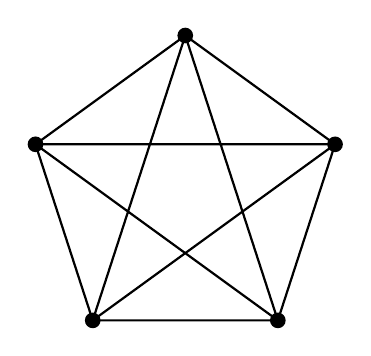
\begin{tikzpicture}
		\draw[thick,black]  (18:2) \foreach \a in {90,162,234,306} { -- (\a:2) } -- cycle;
		\draw[thick,black] (18:2) \foreach \a in {162,306,90,234} { -- (\a:2) } -- cycle;
		\foreach \a in {18,90,162,234,306} { \node[black,fill=black,circle,inner sep=2pt] at (\a:2){}; }
	\end{tikzpicture}
	\caption{完全图}
\end{figure}

\vspace{0.5cm}

\subsection{圈图(Cycle Graph)}

圈图是由$ n\ (n \ge 3) $的顶点,及边$ (v_1, v_2) $、$ (v_2, v_3) $、$ (v_{n-1}, v_n) $、$ (v_n, v_1) $组成的简单图。

\begin{figure}[H]
	\centering
	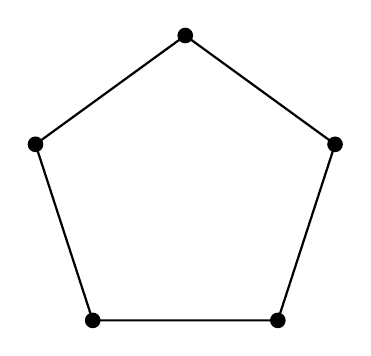
\begin{tikzpicture}
		\draw[thick,black]  (18:2) \foreach \a in {90,162,234,306} { -- (\a:2) } -- cycle;
		\foreach \a in {18,90,162,234,306} { \node[black,fill=black,circle,inner sep=2pt] at (\a:2){}; }
	\end{tikzpicture}
	\caption{圈图}
\end{figure}

\vspace{0.5cm}

\subsection{n立方图}

n立方图记作$ Q_n $,是用顶点表示$ 2^n $个长度为n的二进制串的图。n立方图的两个顶点相邻,当且仅当它们所表示的二进制串恰有一位不同。\\

\begin{figure}[H]
	\centering
	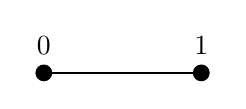
\begin{tikzpicture}
		\node[draw, black, fill=black, circle, inner sep=2pt, label=above:0] at (0,0){};
		\node[draw, black, fill=black, circle, inner sep=2pt, label=above:1] at (2,0){};
		\draw[black, thick] (0,0) -- (2,0);
	\end{tikzpicture}
	\caption{$ Q_1 $}
\end{figure}

\begin{figure}[H]
	\centering
	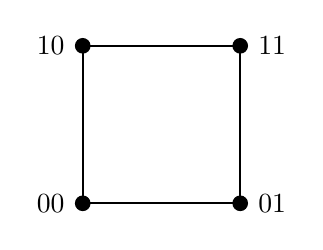
\begin{tikzpicture}
		\node[black, fill=black, circle, inner sep=2pt, label=left:00] at (0,0){};
		\node[black, fill=black, circle, inner sep=2pt, label=right:01] at (2,0){};
		\node[black, fill=black, circle, inner sep=2pt, label=right:11] at (2,2){};
		\node[black, fill=black, circle, inner sep=2pt, label=left:10] at (0,2){};
		\draw[black, thick] (0,0) -- (2,0) -- (2,2) -- (0,2) -- (0,0);
	\end{tikzpicture}
	\caption{$ Q_2 $}
\end{figure}

\begin{figure}[H]
	\centering
	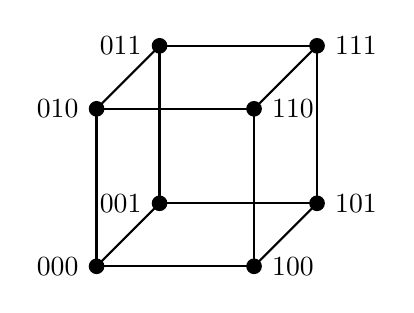
\begin{tikzpicture}
		\node[black, fill=black, circle, inner sep=2pt, label=left:000] at (0,0){};
		\node[black, fill=black, circle, inner sep=2pt, label=right:100] at (2,0){};
		\node[black, fill=black, circle, inner sep=2pt, label=right:110] at (2,2){};
		\node[black, fill=black, circle, inner sep=2pt, label=left:010] at (0,2){};
		\draw[black, thick] (0,0) -- (2,0) -- (2,2) -- (0,2) -- (0,0);

		\node[black, fill=black, circle, inner sep=2pt, label=left:001] at (0.8,0.8){};
		\node[black, fill=black, circle, inner sep=2pt, label=right:101] at (2.8,0.8){};
		\node[black, fill=black, circle, inner sep=2pt, label=right:111] at (2.8,2.8){};
		\node[black, fill=black, circle, inner sep=2pt, label=left:011] at (0.8,2.8){};
		\draw[black, thick] (0.8,0.8) -- (2.8,0.8) -- (2.8,2.8) -- (0.8,2.8) -- (0.8,0.8);

		\draw[black, thick] (0,0) -- (0.8,0.8);
		\draw[black, thick] (0,2) -- (0.8,2.8);
		\draw[black, thick] (2,2) -- (2.8,2.8);
		\draw[black, thick] (2,0) -- (2.8,0.8);
	\end{tikzpicture}
	\caption{$ Q_3 $}
\end{figure}

\vspace{0.5cm}

\subsection{二分图(Bipartite Graph)}

